
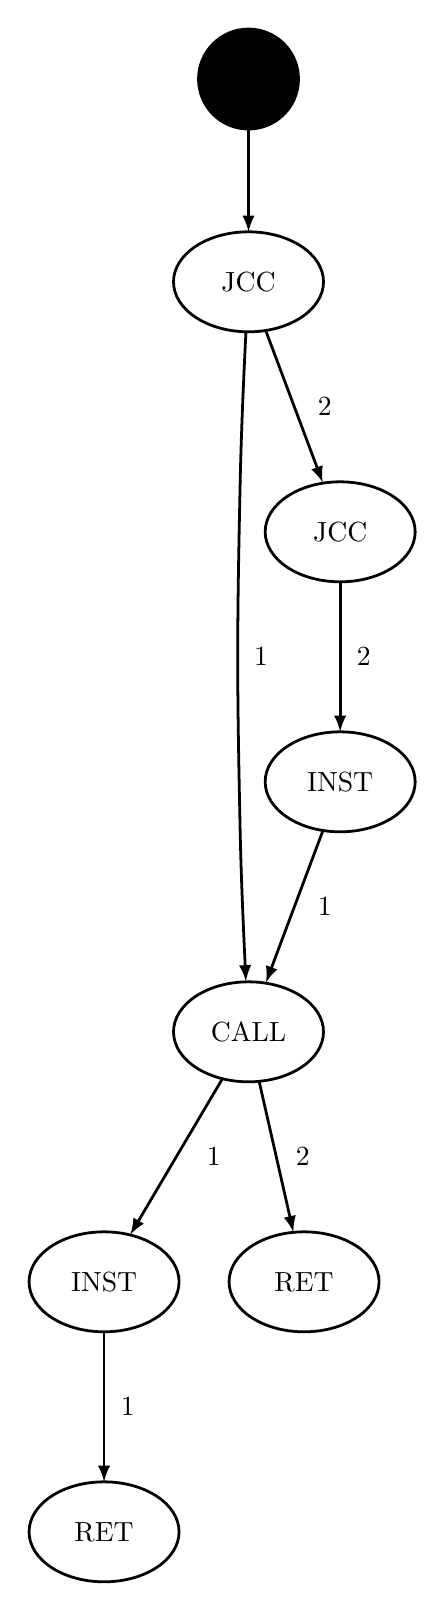
\begin{tikzpicture}[>=latex,line join=bevel,]
  \pgfsetlinewidth{1bp}
%%
\pgfsetcolor{black}
  % Edge: 2 -> 3
  \draw [->] (69.462bp,180.86bp) .. controls (61.693bp,167.71bp) and (50.591bp,148.92bp)  .. (36.477bp,125.04bp);
  \definecolor{strokecol}{rgb}{0.0,0.0,0.0};
  \pgfsetstrokecolor{strokecol}
  \draw (66.5bp,153bp) node {1};
  % Edge: 6 -> 7
  \draw [->] (112bp,359.61bp) .. controls (112bp,347.24bp) and (112bp,330.37bp)  .. (112bp,306.05bp);
  \draw (120.5bp,333bp) node {2};
  % Edge: 1 -> 6
  \draw [->] (85.207bp,450.45bp) .. controls (89.97bp,437.75bp) and (96.639bp,419.96bp)  .. (105.71bp,395.78bp);
  \draw (106.5bp,423bp) node {2};
  % Edge: 7 -> 2
  \draw [->] (105.79bp,270.45bp) .. controls (101.03bp,257.75bp) and (94.361bp,239.96bp)  .. (85.291bp,215.78bp);
  \draw (106.5bp,243bp) node {1};
  % Edge: 1 -> 2
  \draw [->] (78.069bp,449.79bp) .. controls (77.341bp,435.42bp) and (76.388bp,414.38bp)  .. (76bp,396bp) .. controls (74.818bp,340.01bp) and (74.818bp,325.99bp)  .. (76bp,270bp) .. controls (76.303bp,255.64bp) and (76.951bp,239.66bp)  .. (78.069bp,216.21bp);
  \draw (83.5bp,333bp) node {1};
  % Edge: 0 -> 1
  \draw [->] (79bp,522.81bp) .. controls (79bp,514.79bp) and (79bp,505.05bp)  .. (79bp,486.03bp);
  % Edge: 2 -> 5
  \draw [->] (82.856bp,180.03bp) .. controls (85.706bp,167.49bp) and (89.643bp,150.17bp)  .. (95.156bp,125.92bp);
  \draw (98.5bp,153bp) node {2};
  % Edge: 3 -> 4
  \draw [->] (27bp,89.614bp) .. controls (27bp,77.24bp) and (27bp,60.369bp)  .. (27bp,36.05bp);
  \draw (35.5bp,63bp) node {1};
  % Node: 1
\begin{scope}
  \definecolor{strokecol}{rgb}{0.0,0.0,0.0};
  \pgfsetstrokecolor{strokecol}
  \draw (79bp,468bp) ellipse (27bp and 18bp);
  \draw (79bp,468bp) node {JCC};
\end{scope}
  % Node: 0
\begin{scope}
  \definecolor{strokecol}{rgb}{0.0,0.0,0.0};
  \pgfsetstrokecolor{strokecol}
  \definecolor{fillcol}{rgb}{0.0,0.0,0.0};
  \pgfsetfillcolor{fillcol}
  \filldraw [opacity=1] (79bp,541bp) ellipse (18bp and 18bp);
\end{scope}
  % Node: 3
\begin{scope}
  \definecolor{strokecol}{rgb}{0.0,0.0,0.0};
  \pgfsetstrokecolor{strokecol}
  \draw (27bp,108bp) ellipse (27bp and 18bp);
  \draw (27bp,108bp) node {INST};
\end{scope}
  % Node: 2
\begin{scope}
  \definecolor{strokecol}{rgb}{0.0,0.0,0.0};
  \pgfsetstrokecolor{strokecol}
  \draw (79bp,198bp) ellipse (27bp and 18bp);
  \draw (79bp,198bp) node {CALL};
\end{scope}
  % Node: 5
\begin{scope}
  \definecolor{strokecol}{rgb}{0.0,0.0,0.0};
  \pgfsetstrokecolor{strokecol}
  \draw (99bp,108bp) ellipse (27bp and 18bp);
  \draw (99bp,108bp) node {RET};
\end{scope}
  % Node: 4
\begin{scope}
  \definecolor{strokecol}{rgb}{0.0,0.0,0.0};
  \pgfsetstrokecolor{strokecol}
  \draw (27bp,18bp) ellipse (27bp and 18bp);
  \draw (27bp,18bp) node {RET};
\end{scope}
  % Node: 7
\begin{scope}
  \definecolor{strokecol}{rgb}{0.0,0.0,0.0};
  \pgfsetstrokecolor{strokecol}
  \draw (112bp,288bp) ellipse (27bp and 18bp);
  \draw (112bp,288bp) node {INST};
\end{scope}
  % Node: 6
\begin{scope}
  \definecolor{strokecol}{rgb}{0.0,0.0,0.0};
  \pgfsetstrokecolor{strokecol}
  \draw (112bp,378bp) ellipse (27bp and 18bp);
  \draw (112bp,378bp) node {JCC};
\end{scope}
%
\end{tikzpicture}

